\chapter{Mathematical Preliminaries}
\label{chapter:mathematical-preliminaries}

This chapter is intended to serve as a reference point, clarifying ideas and notation for the more fundamental concepts that will be used throughout the remainder of this dissertation. In the first section we discuss order and lattice theory. The third and final section introduces propositional logic, as well more general ideas in logic.

\section{Order and Lattice Theory}
\label{section:order-theory}

This section refers extensively to the fundamental text by Davey and Priestley \cite{davey2002introduction}, as well as Ganter and Wille \cite{ganter1999formal}.

\subsection{Orders}
\label{subsection:orders}

A \textit{binary relation} \index{binary relation} $R$ over the sets $X$ and $Y$ is a set of ordered pairs $\op{x,y}$ where $x \in X$ and $y \in Y$. We may choose to express $\op{x,y} \in R$ using infix notation and write $xRy$, which tells us that $R$ relates $x$ to $y$.
 
Certain binary relations, satisfying specific properties, occur frequently enough to warrant their own denomination. One such relation, which will be used in almost every section of this dissertation, is called a \textit{partial order}.

\begin{definition}
  \label{definition:partial-order}
  A \textit{partial-order} \index{partial-order} is a binary relation $\preceq \; \subseteq X \times X$ that satisfies the following properties:
  \begin{align}
    \text{(Reflexivity)} \quad & x \preceq x \\
    \text{(Antisymmetry)} \quad & x \preceq y \text{ and } y \preceq x \text{ implies } x = y \\
    \text{(Transitivity)} \quad & x \preceq y \text{ and } y \preceq z \text{ implies } x \preceq z
  \end{align}
  for all $x,y,z \in X$.
\end{definition}

Frequently, `preference' is used as a metonymy for an order, and so in this context \say{element $x$ is preferred to $y$} should be taken to mean that $\op{x,y} \in \; \preceq$, or simply $x \preceq y$.

We write $x \npreceq y$ to indicate that $\op{x,y}$ is not in the relation, and $x \prec y$ for the case where $x\preceq y$ and $x \not = y$. In the scenario where $x \not \preceq y$ and $y \not \preceq x$---i.e., that $x$ and $y$ are incomparable---we write $x \Vert y$. From a partial-order we can quite easily induce the notion of a \emph{strict partial-order}.

\begin{definition}
  \label{definition:strict-partial-order}
  A \textit{strict partial-order} \index{partial-order! strict partial-order} is a binary relation $\prec \; \subseteq X \times X$ that satisfies:
  \begin{align}
     \text{(Irreflexivity)} \quad & x \nprec x \\
     \text{(Asymmetry)} \quad & x \prec y \text{ implies } y \nprec x \\
     \text{(Transitivity)} \quad & x \prec y \text{ and } y \prec z \text{ implies } x \prec z
  \end{align}
  for all $x,y,z \in X$.
\end{definition}

An \textit{ordered set} is a pair $(X, \preceq)$ with $X$ being a set and $\preceq$ being an ordering on the elements of $X$. We make notation easier, and use $\mathbf{X}$ to denote the pair; moreover, the order relation associated with $\mathbf{X}$ may be written $\preceq_X$ in settings where ambiguity arises. If $\mathbf{Y}$ is a subset of $\mathbf{X}$, then $\mathbf{Y}$ inherits the order relation from $\mathbf{X}$; and so, for $x,y \in \mathbf{Y}$, $x \preceq_Y y$ if and only if $x \preceq_X y$.

We can visualize ordered sets through the use of \textit{Hasse} diagrams\index{Hasse diagrams}.

\begin{figure}[H]
  \centering
  \small
  \begin{subfigure}{0.3\textwidth}
    \centering
    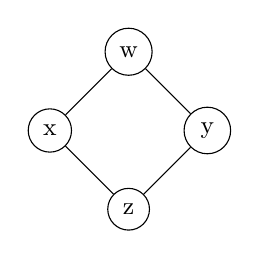
\begin{tikzpicture}[every node/.style={circle, draw, minimum size=0.1cm, font=\small}]
      \node (w) at (0,1) {w};
      \node (y) at (-1,0) {x};
      \node (z) at (1,0) {y};
      \node (x) at (0,-1) {z};

      \draw (w) -- (y);
      \draw (w) -- (z);
      \draw (y) -- (x);
      \draw (z) -- (x);
    \end{tikzpicture}
    \subcaption{$\mathbf{A}$}
    \label{subfigure:partial-order-a}
  \end{subfigure}%
  \begin{subfigure}{0.3\textwidth}
    \centering
    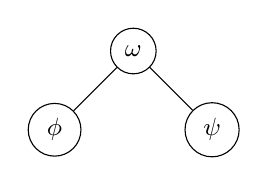
\begin{tikzpicture}[every node/.style={circle, draw, minimum size=0.1cm, font=\small}]
      \node (y) at (-1,0) {$\phi$};
      \node (z) at (1,0) {$\psi$};
      \node (x) at (0,1) {$\omega$};

      \draw (y) -- (x);
      \draw (z) -- (x);
    \end{tikzpicture}
    \subcaption{$\mathbf{B}$}
    \label{subfigure:partial-order-b}
  \end{subfigure}%
  \caption{Hasse diagrams of two partially ordered sets}
  \label{figure:hasse-diagram}
\end{figure}

As an illustrative example, from the ordered set in \Cref{subfigure:partial-order-a} we read that $z \preceq x$, as there is a (strictly) upward path from $z$ to $x$. In fact, it is clear that $z \preceq w, x,y,z$, or that \say{$z$ is preferred to every other element in $\mathbf{A}$}. We say such an element is \textit{minimal}.

More formally, an element $x \in \mathbf{X}$ is \textit{minimal} with respect to the ordering if there exists no distinct element $y \in \mathbf{X}$ such that $y \preceq x$. Conversely, we say $x$ is \textit{maximal} if there exists no distinct $y \in \mathbf{X}$ where $x \preceq y$. Then $x$ is the \textit{minimum} element if $x \preceq y$ for all $y \in \mathbf{X}$; the dual notion of a \textit{maximum} is defined as we might expect. \index{maximum} \index{minimum} \index{maximal} \index{minimal}

\begin{definition}
  \label{definition:order-maps}

     \index{map! order-preserving} \index{map! order-embedding} \index{map! order-isomorphism}
  Let $\mathbf{X}$ and $\mathbf{Y}$ be ordered sets with a mapping $\varphi : \mathbf{X} \to \mathbf{Y}$. We call $\varphi$ an \textit{order-preserving} (or, isotone) map if $x \preceq_X y$ implies $\varphi(x) \preceq_Y \varphi(y)$. It is an \textit{order-embedding} if it is injective, and $x \preceq_X y$ if and only if $\varphi(x) \preceq_Y \varphi(y)$ for all $x,y \in X$. Finally, $\varphi$ is an \textit{order-isomorphism} if it is an order-embedding that is also \textit{surjective}. The dual notion to an order-preserving map is an \textit{order-reversing} (or, antitone) map. \index{order-reversing map}
\end{definition}

\subsection{Lattice Theory}
\label{subsection:lattice-theory}
Lattice theory studies partially ordered sets that behave well with respect to upper and lower bounds. Given an ordered set $\mathbf{X}$ and a subset $\mathbf{Y} \subseteq \mathbf{X}$, the set of upper bounds of $\mathbf{Y}$ is defined as
\[
  \mathbf{Y}^u \coloneqq \{x \in \mathbf{X} \mid \forall y \in \mathbf{Y} : y \preceq x\},
\]
and the set of lower bounds, $\mathbf{Y}^l$, is defined dually. If $\mathbf{Y}^u$ has a minimum element, then we call that element the \textit{supremum} of $\mathbf{Y}$; dually, if $\mathbf{Y}^l$ has a maximum element, then we call that element the \textit{infimum} of $\mathbf{Y}$. Instead of talking about the supremum of two elements $x,y \in \mathbf{X}$, we opt for the term \textit{join} and write $x \vee y$, or $\bigvee \mathbf{Y}$ where $\mathbf{Y} \subseteq \mathbf{X}$. Instead of infimum, we say \textit{meet} and write $x \wedge y$, or $\bigwedge \mathbf{Y}$. \index{upper bound} \index{lower bound} \index{join} \index{meet}

A \textit{lattice} is a non-empty partially ordered set $\mathbf{L}$ in which every pair of elements $x,y \in \mathbf{L}$ for which $x \wedge y$ and $x \vee y$ exists. If $\bigwedge \mathbf{M}$ and $\bigvee \mathbf{M}$ exist for any subset $\mathbf{M} \subseteq \mathbf{L}$ then $\mathbf{L}$ is a \textit{complete lattice}. \index{lattice} \index{lattice! complete lattice} 

% \begin{example}
%   \label{example:lattice of naturals}
%   The set $\mathbb{N}$ of natural numbers forms a complete lattice when ordered by divisibility. In this lattice, the meet and join operations correspond to the greatest common divisor and least common multiple, respectively. The bottom element of the lattice is $1$, as it divides all natural numbers; while the top element is $0$ since it divides every natural.
% \end{example}

\subsubsection{Lattices as algebraic structures}
\label{subsubsection:lattices-as-algebraic-structures}

From another perspective, a lattice can be seen as an algebraic structure where meet and join are binary operations on a set. Then, $\langle L, \vee, \wedge \rangle$ formally represents a lattice. Often, we simplify notation to just $L$ when the context clearly indicates the operations.

If the set $L$ is equipped with only one of these operations, the structure is called a \textit{semilattice}. Specifically, the structure $\langle L, \vee \rangle$ (resp. $\langle L, \wedge \rangle$) is called a \textit{join semilattice} (resp. a \textit{meet semilattice}). Such a structure is a reduct of a lattice, satisfying the following properties for all $x, y, z \in L$:

\vspace{-1em}
\begin{align}
     \text{(associative)} & \quad (x \vee y) \vee z = x \vee (y \vee z) & \quad \text{(resp.)} & \quad (x \wedge y) \wedge z = x \wedge (y \wedge z) \\ \index{Boolean operator! associativity} 
  \text{(commutative)} & \quad x \vee y = y \vee x & \text{(resp.)}  & \quad x \wedge y = y \wedge x \\ \index{Boolean operator! commutativity}
  \text{(idempotent)}  & \quad x \vee x = x & \text{(resp.)}  & \quad x \wedge x = x \index{Boolean operator! idempotency}
\end{align}

Finally, when considering both operations simultaneously, the interaction between join and meet operations within a lattice structure is governed by the absorption laws:

\vspace{-1em}
\begin{align}
  \text{(absorption)} & \quad x \vee (x \wedge y) = x & \text{(resp.)}  & \quad x \wedge (x \vee y) = x
\end{align}

\begin{figure}[H]
  \centering
  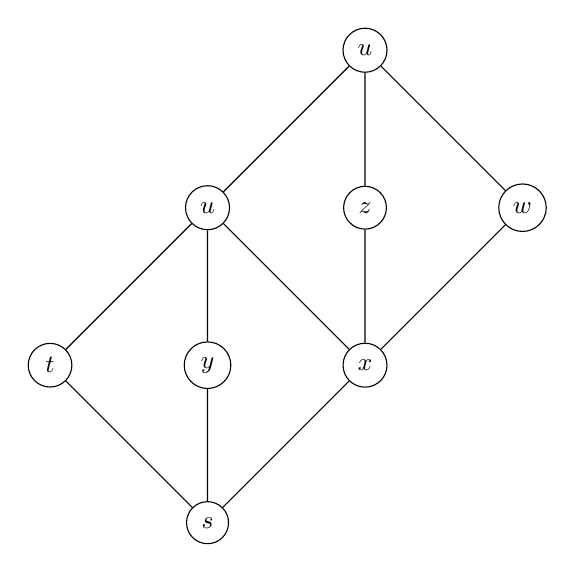
\begin{tikzpicture}[every node/.style={circle, draw, minimum size=0.05cm, font=\small}]
    \node (s) at (-1,-2) {$s$};
    \node (t) at (-3,0) {$t$};
    \node (u) at (-1,2) {$u$};
    \node (v) at (1,4) {$u$};
    \node (w) at (3,2) {$w$};
    \node (x) at (1,0) {$x$};
    \node (y) at (-1,0) {$y$};
    \node (z) at (1,2) {$z$};

    \draw (s) -- (t) -- (u) -- (v) -- (w) -- (x) -- (s);
    \draw (s) -- (y) -- (u) -- (x) -- (z) -- (v);
  \end{tikzpicture}
  \caption{A complete lattice}
  \label{figure:complete-lattice}
\end{figure}

\Cref{figure:complete-lattice} illustrates a simple complete lattice; verifying that arbitrary meets and joins exist for all subsets. There is an obvious similarity between this representation of a lattice and the Hasse diagrams in \Cref{figure:hasse-diagram} used to describe partially ordered sets. This is perhaps obvious, given the opening remarks where we described a lattice as an ordered set, satisfying certain properties on upper and lower bounds. However, \Cref{lemma:the-connecting-lemma} makes the connection between the order and algebraic views of lattices concrete.

\begin{lemma}[The Connecting Lemma]
  \label{lemma:the-connecting-lemma}
  If $\mathbf{L}$ is a lattice with $x, y \in \mathbf{L}$, then the following are equivalent:
  \begin{enumerate}
      \setlength\itemsep{0pt}
      \setlength\parsep{0pt}
    \item $x \preceq y$;
    \item $x \vee y = y$;
    \item $x \wedge y = x$.
  \end{enumerate}
\end{lemma}

Moving forward, we will no longer keep the order‑theoretic and algebraic perspectives on lattices strictly separate; rather, we will tacitly adopt whichever viewpoint best suits the surrounding context. Lattices are central to Formal Concept Analysis and will be revisited in \Cref{chapter:formal-concept-analysis}.

\section{Propositional Logic}
\label{section:propositional-logic}

Propositional logic is a system for abstracting reasoning away from natural language. A \textit{propositional statement} is a claim like \say{Tralfamadorians have one eye}; that is, something that can be assigned a value of \textit{true} or \textit{false} \cite[p. 7]{Ben1993Mathematical}. More complex statements can be recursively constructed from simpler ones; our interest is then about which propositions follow from others. 

\subsection{Syntax}
\label{subsection:syntax}
\index{syntax! propositional logic} \index{Atom} \index{Propositional atom} \index{Boolean operator} \index{Boolean operator! and} \index{Boolean operator! or} \index{Boolean operator! material implication} \index{Boolean operator! negation}
\textit{Propositional atoms} are the construction blocks of a propositional language. They are indivisible statements that can either be true or false, and maybe be combined with the boolean connectives $\{\neg, \lor, \land, \rightarrow\}$ to construct more complex statements, or \textit{formulae}. We denote propositional atoms with lower-case letters $p,q,r,s,$ and $t$, and formulae with lower-case Greek letters $\alpha, \beta, \gamma, \phi, \psi,$ and $\varphi$. 

Not all combinations of atoms and boolean connectives result in meaningful expressions (for example, `$\land \rightarrow \phi$' has no discernible meaning) and so we make a distinction between any formulae and \textit{well-formed formulae}. The latter being constructions that are valid with respect to the rules of the grammar defined in Backus-Naur form below. We are entirely uninterested in formulae that are not well-formed formulae, and so we drop the `well-formed' suffix with the recognition that we shall never again mention the alternative \cite[p. 33]{Huth_Ryan_2004}.

\begin{align}
  \phi ::= p \mid (\neg \phi) \mid (\phi_1 \lor \phi_2) \mid (\phi_1 \land \phi_2) \mid (\phi_1 \rightarrow \phi_2) \mid (\phi_1 \leftrightarrow \phi_2)
\end{align}

Any formula accepted by this grammar is said to be in the language $\mathcal{L}^\mathcal{P}$, although we will drop the superscript where possible.
To make reading this dissertation slightly more enjoyable, we may construct examples where we denote propositional atoms by monospaced text, enabling the expression of formulae like $\texttt{tralfamadorians} \rightarrow \neg \texttt{human}$, which should be interpreted as meaning \say{Tralfamadorians are not human}.

\subsection{Semantics}
\label{subsection:semantics}
\index{semantics! propositional logic}
In the previous section we described the syntax of propositional logic and how the boolean connectives enable the construction of arbitrary formulae from atoms. The semantics of propositional logic are concerned with how meaning can be ascribed to these formulae. The aim is to provide a method of answer questions like \say{when is this formula true?} or, \say{if $\phi, \psi, \varphi$ are true, what else must be true?}.

Propositional atoms were described as indivisible statements that can be assigned values of \textit{true} or \textit{false}. We now define a function that assigns a truth value to each proposition in the set $\mathcal{P}$ of propositions, sometimes called the \textit{universe of discourse}. \index{valuations}

\begin{definition}
  \label{definition:valuation} \index{valuations} 
  A \textit{valuation} is a function \(u : \mathcal{P} \to \{\textit{ true}, \textit{ false }\}\) that assigns a truth value to each propositional atom.
\end{definition}

Given a set of atoms $\mathcal{P} = \{p,q,r\}$, we write $\mathcal{U}$ to denote the set of all possible valuations. A valuation $u \in \mathcal{U}$ \textit{satisfies} an atom $p \in \mathcal{P}$ if $u$ maps $p$ to \textit{true}, then we write $u \Vdash p$. Otherwise, we write $u \nVdash p$ to indicate that $u$ does not satisfy $p$ (in this context, meaning $u$ maps $p$ to \textit{false}) \cite[p. 16]{Ben1993Mathematical}. We might represent the valuation that maps $p$ and $q$ to true but $r$ to false by $\{p,q,\overline{r}\}$.

This satisfaction relation can be extended beyond propositional atoms to include more complex formulae, as described in \Cref{subsection:syntax}. For any $\phi, \psi \in \mathcal{L}$ \index{satisfaction! propositional logic}

\begin{itemize}
  \item $u \Vdash \neg \phi$ if and only if $u \nVdash \phi$
  \item $u \Vdash \phi \vee \psi$ if and only if $u \Vdash \phi$ or $u \Vdash \psi$
  \item $u \Vdash \phi \wedge \psi$ if and only if $u \Vdash \phi$ and $u \Vdash \psi$
  \item $u \Vdash \phi \rightarrow \psi$ if and only if $u \Vdash \neg \phi$ or $u \Vdash \psi$
  \item $u \Vdash \phi \leftrightarrow \psi$ if and only if $u \Vdash \phi \rightarrow \psi$ and $u \Vdash \psi \rightarrow \phi$
\end{itemize}

\begin{definition} 
  \label{definition:model}
  \index{model}
  For a valuation $u \in \mathcal{U}$ and formula $\phi \in \mathcal{L}$ we call $u$ a \textit{model} of $\phi$ if and only if $u$ satisfies $\phi$. The set of models of $\phi$ is constructed by $\hat{\phi} \coloneqq \{u \in \mathcal{U} \mid u \Vdash \phi \}$.
\end{definition}

Satisfiability can be extended to sets of of formulae so that a valuation $u \in \mathcal{U}$ \textit{satisfies} the set $\Phi \coloneqq \{\phi_0, \ldots, \phi_n \}$ when $u \Vdash \phi_i$ for all $0 \leq i \leq n$, and we write $u \Vdash \Phi$. If no such valuation exists then $\Phi$ is unsatisfiable \cite[p. 31]{Ben1993Mathematical}. 

\subsection{Logical Consequence}
\label{subsection:logical-consequence}
\index{Logical consequence! propositional logic}

The introduction of models at the end of \Cref{section:propositional-logic} leads quite naturally into a discussion on the matter of \textit{logical consequence}, which provides an answer to the question of when it is appropriate to infer one formula from another  \cite[p. 408]{turquette1957logic}.  

For example, if we know that \say{\textit{Billy lived in Slaughterhouse 5}} and that \say{\textit{The inhabitants of Slaughterhouse 5 survived the bombing of Dresden}}. We may then hold the view that, as a consequence of these two pieces of knowledge, it would be sensible to infer that \say{\textit{Billy survived the bombing of Dresden}}. Of course, this inference being \textit{sensible}---under some common concept of consequence---gives little insight into how logical consequence may be appropriately be formalised. 

\index{object language} \index{metalanguage}
We place a brief moratorium on this discussion to (formally) introduce the notions of the \textit{object} and \textit{metalanguage}. In the scenario we have just described, the italicised sentences from a part of the object language: the language we use to model the world and represent information. The metalanguage facilitates reasoning about elements in the object language; that is, we can use the metalanguage to describe one sentence being a consequence of another (where these sentences are elements in the object language). Here, \textit{consequence} is an element of the metalanguage \cite[p 22]{Ben1993Mathematical}.

In this case, both the object and metalanguage are comprised of English which can certainly lead to confusion. It is more common to use a language like the one described in \Cref{subsection:syntax} as the object language, and a metalanguage comprising of symbols like $\vDash$ and $\vdash$, which we introduce below. 

\begin{definition}
     \label{definition:logical-consequence}
     Let $\Gamma$ be a set of formulae and $\varphi$ a formula in the language $\mathcal{L}$. We say that $\varphi$ is a \textit{logical consequence} of $\Gamma$, and write $\Gamma \vDash \varphi$, if and only if every model of $\Gamma$ is a model of $\varphi$, or equivalently if $\hat{\Gamma} \subseteq \hat{\varphi}$.
\end{definition}

Logical consequence can be used to define an operator $\mathcal{C}n$ such that if $\Gamma$ is a set of formulae in $\mathcal{L}$, then $\mathcal{C}n(\Gamma) \coloneqq \{\alpha \in \mathcal{L} \mid \Gamma \vDash \alpha\}$

\begin{example}
     \label{example-logical-consequence}   
Let us model the earlier scenario in propositional logic, and so we now initialise \textit{Billy} with \texttt{b}, \textit{slaughterhouse 5} with \texttt{h}, and \textit{survived} with \texttt{s}. The ``sensible inference'' we posed was to determine whether $\texttt{b} \rightarrow \texttt{s}$ should---under some reasonable account of consequence---follow from the set $\{\texttt{b} \rightarrow \texttt{h},\; \texttt{h} \rightarrow \texttt{s}\}$. 
\end{example}


\subsection{Deductive Systems}
\label{subsection:deduction-systems}
\index{Deductive system} \index{Rule of inference} \index{Axiom}
Logical consequence, described in \Cref{subsection:logical-consequence}, offers a purely semantic account of how it might be inferred that one formula follows (logically) from another set thereof. In contrast, deductive systems answer this question syntactically by describing a system of \textit{axiomata} and \textit{rules of inference}. 

\begin{definition}
     \label{definition:deductive-system} 
     A \textit{deductive system} is a collection of axiomata and rules of inference. A \textit{proof} in such a system is a sequence of formulae where each formula is either an axiom, or has been inferred by application of an inference rule to previous formulae in the sequence. The final formula in the sequence, $\phi$, is called the \textit{theorem} and is \textit{provable}, and so we write $\vdash \phi$. 
\end{definition}

Deductive systems offer some advantages over their semantic counterparts; particularly, when reasoning over large---possibly infinite---domains, logical consequence can become difficult. Moreover, semantic consequence provides little insight into the relationships between pieces of information that lead to the inferences we make; while the sequential nature of deduction systems trace a path describing this relationship \cite[p. 55]{Ben1993Mathematical}.

\subsubsection{Hilbert Systems} 
\label{subsubsection:hilbert-systems}
\index{Deductive system! Hilbert system}

A propositional Hilbert system $\mathcal{H}$ is characterised by three axiom schemata, \index{Axiom scheme}
\begin{align}
    \text{(Axiom 1)} \quad & \vdash (\phi \rightarrow (\psi \rightarrow \phi)),  \\ 
    \text{(Axiom 2)} \quad & \vdash (\phi \rightarrow (\psi \rightarrow \gamma)) \rightarrow ((\phi \rightarrow \psi) \rightarrow (\phi \rightarrow \gamma)), \\
    \text{(Axiom 3)} \quad & \vdash (\neg \phi \rightarrow \neg \psi) \rightarrow (\phi \rightarrow \psi),
\end{align}
%
and a single rule of inference:
%
\begin{align}
     \index{Rule of inference! \textit{modus ponens}}
     \text{(Modus Ponens)} \quad & \frac{\vdash \phi, \qquad \vdash \phi \rightarrow \psi}{\vdash \psi}.
\end{align}
%
The axiom schemata themselves are not axioms, but rather patterns containing meta-variables that, when uniformly substituted for formulae, result in an axiom. The turnstile symbol ($\vdash$) is the syntactic counterpart to the double-turnstile ($\vDash$) used for logical consequence. We frequently express that $\phi$ is a theorem by writing $\vdash \phi$ \cite[p. 55]{Ben1993Mathematical}.

As it stands, constructing proofs from instances of axiom schema and applications of modus ponens is a challenging ordeal. \textit{Derived rules} are introduced as a means to make it easier to spot the next step in a proof sequence. Of particular importance is the so called \textit{deduction theorem}; which allows the construction of proofs that are conditioned on a hypothesis, without requiring that the hypothesis be an axiom. \index{Rule of inference! deduction}
%
\begin{align}
     \text{(Deduction Theorem)} \quad & \frac{\Delta \cup \phi \vdash \psi}{\Delta \vdash \phi \rightarrow \psi}
\end{align}
%
Derived rules must be sound with respect to what can be proved by the three axioms and applications of modus ponens. That is, a derived rule should not enable one to make an inference that would not be possible without such a rule. 

As an illustration, we provide the following Hilbert-style proof for the inference made in \Cref{example-logical-consequence}. 

\begin{theorem}
\(
  \texttt{b} \rightarrow \texttt{h},\;
  \texttt{h} \rightarrow \texttt{s}
  \;\vdash\;
  \texttt{b} \rightarrow \texttt{s}
\)
\end{theorem}
%
\begin{proofH}
  \Hstep[Premise]{\vdash (\texttt{b} \rightarrow \texttt{h})}
  \Hstep[Premise]{\vdash (\texttt{h} \rightarrow \texttt{s})}
  \Hstep[Axiom 1]{\vdash (\texttt{h} \rightarrow \texttt{s}) \rightarrow (\texttt{b} \rightarrow (\texttt{h} \rightarrow \texttt{s}))}
  \Hstep[MP 2,3]{\vdash (\texttt{b} \rightarrow (\texttt{h} \rightarrow \texttt{s}))}
  \Hstep[Axiom 2]{\vdash (\texttt{b} \rightarrow (\texttt{h} \rightarrow \texttt{s})) \rightarrow ((\texttt{b} \rightarrow \texttt{h}) \rightarrow (\texttt{b} \rightarrow \texttt{s}))} 
  \Hstep[MP 4,5]{\vdash (\texttt{b} \rightarrow \texttt{h}) \rightarrow (\texttt{b} \rightarrow \texttt{s})}
  \Hstep[MP 1,6]{\vdash (\texttt{b} \rightarrow \texttt{s})}
\end{proofH} 

\subsubsection{Gentzen Systems} 
\label{subsubsection:gentzen-systems}
\index{Genzten systems}

\subsection{Soundness and Completeness} 
\label{subsection:soundness-and-completeness}
\index{soundness! propositional logic! Hilbert system} \index{soundness! propositional logic! Gentzen system} \index{completeness! propositional logic! Gentzen system} \index{completeness! propositional logic! Hilbert system}

\subsection{Consequence Relations} 
\label{subsection:consequence-relations}
\index{consequence relations}

